%%%%%%%%%%%%%%%%%%%%%%%%%%%%%%%%
\subsection{Objetivo}
% ----------------------------------------------------------------------------
\begin{frame}{Reconhecimento de Voz}

\begin{figure}
	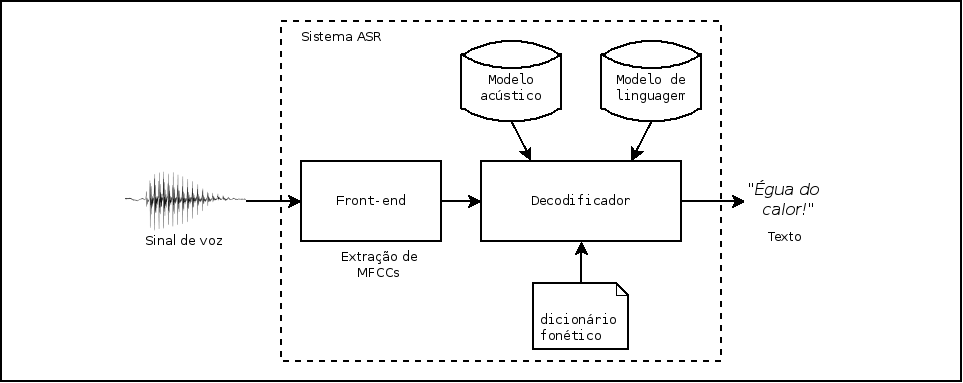
\includegraphics[width=0.9\textwidth]{Figures/asr}
    \caption{Esquema tradicional de um sistema autom\'atico de reconhecimento de voz}
\end{figure}

\begin{itemize}
    \item Aplica\c c\~oes:
    \begin{itemize}
        \smallskip
		\item Tecnologias assistivas, \textit{eye-trackers}, lingu\'istica (\textbf{alinhamento fon\'etico}), s\'intese de voz
    \end{itemize}
\end{itemize}
\end{frame}


\begin{frame}
\frametitle{Alinhamento Fon\'etico For\c cado}
	\begin{itemize}
		\item Automatiza\c c\~ao  da transcri\c c\~ao e alinhamento de fala gravada
		\item Estudo e pesquisa de linguistas
		\item Desenvolvimento de ferramentas mais robustas de reconhecimento e sintese de fala
	\end{itemize}
	\begin{figure}
	\begin{center}
		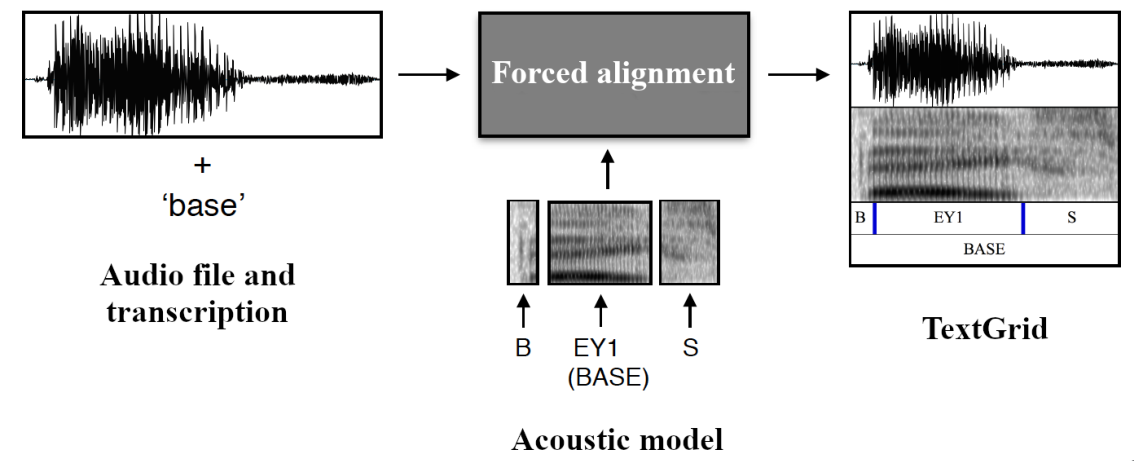
\includegraphics[width=0.8\textwidth]{Figures/align}
	\end{center}
	\end{figure}


\end{frame}


\begin{frame}{Ferramentas}
    \begin{itemize}
        \item Kaldi: um pacote \textit{open-source} de reconhecimento de voz
			\begin{itemize}
				\item Possui suporte para ambas HMM-GMMs (mistura de gaussianas) e HMM-DNNS (redes neurais profundas)
				\item Suporte para PT-BR
			\end{itemize}
		\begin{figure}
		\begin{center}
			
\includegraphics[width=0.4\textwidth]{Figures/kaldi}
		\end{center}
		\end{figure}

        \item Praat: \textit{software} utilizado por linguistas na  an\'alise da fala


        \item UFPAlign: alinhador fon\'etico autom\'atico baseado no HTK disponilizado pelo grupo Fala Brasil
    \end{itemize}
\end{frame}


\begin{frame}{Objetivo}
\begin{itemize}
    % \item Desenvolver um sistema de reconhecimento de voz para PT\_BR utilizando o pacote Kaldi para treinamento dos AMs e LMs
	\item Desenvolver um alinhador fon\'etico para PT\_BR baseado nos modelos
        ac\'usticos explorados no projeto anterior utilizando o Kaldi
	\begin{itemize}
		\item \textit{Plug-in} para o Praat
		\item Modelos ac\'usticos (AMs) treinados utilizando DNNs e HMM-GMMs
	\end{itemize}
	% \item Coletar dados para realizar \textit{LM rescoring}: 4-5 milh\~oes de frases
	\item Substituir o HTK na antiga ferramenta utilizada pelo grupo Fala
        Brasil com o objetivo de melhorar os resultados obtidos
    \item Disponibilizar recursos \`a comunidade cient\'ifica: grupo Fala Brasil
\end{itemize}

\begin{figure}
\begin{center}
	
\includegraphics[width=0.3\textwidth]{Figures/falabrasil}
\end{center}
\end{figure}

\end{frame}
